% -*- root: ../main.tex -*-
%!TEX root = ../main.tex
% this file is called up by main.tex
% content in this file will be fed into the main document
% vim:textwidth=80 fo=cqt

\glsreset{rom}

Battery modellers face the classic  conundrum of conjuring physics-based battery
models that remain amenable for control  applications. The prior attempts by the
research  community  to  tackle  this  challenge  is  examined  here.  The  term
`control-oriented model' can  be considered synonymous with  the term \gls{rom}.
This is  due to the  fact that the  inherent complexity of  physics-based models
inherently  necessitates the  use of  some  order reduction  strategy for  their
adoption in  control and real-time  applications. In this  thesis as well  as in
the  relevant  literature  discussed  here,  these  two  terms  have  been  used
interchangeably.

Research into  \glspl{rom} is  motivated by  the pressing  need for  a real-time
model  with accuracy  properties of  full-order \glspl{pbm}  but possessing  the
computational  simplicity of  equivalent-circuit models  (see~\cref{subsec:ecms}
and~\cref{subsec:pbms} for  an overview). A  number of approaches to  reduce the
computational  complexity of  the  physics-based models  have  been explored  in
literature. Jokar~\etal~\cite{Jokar2016}  provide a comprehensive review  of the
various categories of reduced order  physics based battery models. However, this
work  does  not aim  to  classify  models  based on  time-vs-frequency  domains.
Fan~\etal{}~\cite{Fan2015}  conducted  a  review   of  reduced  order  modelling
methods, but only provide a generic overview of deriving and implementing models
in these  dual domains  without an  expository analysis  of the  implications of
these modelling  choices. Unlike  Jokar~\etal~\cite{Jokar2016}, this  review did
not aim to provide a classification of various reduced order models, but instead
emphasises  on  a broad  survey  of  relevant  methodologies and  tools  towards
\emph{obtaining} them.  Hence, neither  of these works  provide an  insight into
the  rubrics and  implications  of the  choice  of either  of  these domains  to
underpin  the  \glspl{rom}. Although  in  principle  the transformation  between
them  is  often  a straightforward  mathematical  exercise,  \fxnote{citation(s)
needed?}availability of models for final  implementation in the time domain aids
immediate uptake by  industry for adoption in online  \glspl{bms}. The treatment
of \gls{rom} from  this aspect is so  germane to the central  hypothesis of this
chapter,\fxnote{``can a simple time domain model  do the job?''} that the author
of this thesis feels compelled to undertake a simpler classification exercise of
the existing modelling  art, within the context of their  suitability for online
implementation.


In this discussion,  various modelling methodologies and  their resultant models
are viewed as  a single continuum. Consequently this thesis  discusses them from
such a  unified perspective without  microscopic separation of the  final models
from their progenitor mathematical methods. Furthermore, there is also a need to
highlight the salient works among the more recent advances and extensions to the
then  prevailing models  to obtain  an updated  view of  the modelling  art that
have  gained  traction  since the  publication  of  Jokar~\etal~\cite{Jokar2016}
and  Fan~\etal~\cite{Fan2015}. Hence,  the specialised  review of  reduced order
modelling  literature covered  in this  section  intends to  supplement ---  not
supplant --- the breadth of research covered between these works. In particular,
care has been taken to minimize repetition of background art already analysed in
these aforementioned review  articles, thereby striving to report  the subset of
prior research  that is  pertinent to illustrate  the new  classification scheme
introduced  here.  The  author  does  not  aim  to  adhere  to  a  chronological
presentation of such  background works. Instead, salient  \gls{rom} families are
usually  introduced in  the context  of discussing  their significance  within a
particular mathematical modelling technique.


In the views of this thesis author, physics-based control-oriented models can be
classified as belonging to one of the following categories:
\begin{itemize}
    \item Frequency domain \glsfmtshort{rom}s
    \item Quasi-hybrid time/frequency domain \glsfmtshort{rom}s
    \item Hybrid \glsfmtshort{rom}s based on equivalent circuits
    \item Time-domain \glsfmtshort{rom}s
\end{itemize}
It is important to distinguish between those models that are derived directly in
the time  domain versus  those that  are derived first  in the  frequency domain
and  later  converted  to  time  domain.  \fxnote{enumerate  all  the  desirable
characteristics and criterion upon which models are to be evaluated}


In  principle, any  modelling  method  that yields  a  time domain  mathematical
description of physical  phenomena that is lower in  computational complexity by
an arbitrary  magnitude than the original  \gls{dfn} model can be  considered as
a  candidate  for further  investigation.  In  the  absence  of a  canonical  or
quantitative definition of what constitutes a reduced order model, the number of
candidate family  of models  to consider is  overwhelmingly large.  In practice,
the  constraints and  challenges  imposed  by the  scope  of  this work,  \viz{}
suitability  for  real-time  implementation,  limits  the  choice  of  candidate
modelling  families.  For  instance,   models  relying  primarily  on  classical
finite  difference~\cite{Smith2006}, Galerkin's  approximation~\cite{Dao2012} or
Galerkin's  projection~\cite{Fan2016,Fan2018}  methods  for  transformation  and
order  reduction of  one or  more  field variables  of the  \gls{dfn} model  are
excluded from  further study. This  is done in  view of the  impracticability of
implementing  such  models in  a  resource-constrained  environment such  as  an
embedded \gls{bms} controller.

\subsection{Frequency   domain   \glsfmtshort{rom}s}\label{subsec:freqdomainroms}

Owing  to the  low entry-barrier  for adoption  in a  real-time controller  that
typically  logs data  samples at  specific time  intervals, this  thesis focuses
exclusively on models that are cast in a mathematical form directly suitable for
final implementation  in the time domain.  This choice implies the  exclusion of
those models that are derived and  implemented entirely in the frequency domain.
For the sake  of readers interested in frequency domain  methods, the discussion
here  briefly introduces  salient literature  employing the  Padé approximation
method that serves as a backbone of a wide variety of frequency domain models.


The     transfer     function     oriented    Padé     approximation     method
for    low    order    physics-based     battery    modelling    pioneered    by
Forman~\etal{}~\cite{Forman2011a}    has   gained    widespread   adoption    in
the    areas     of    cell     design~\cite{Marcicki2013},    charge-trajectory
optimisation~\cite{Bashash2010},    controller    design~\cite{Perez2015}    and
state    estimation~\cite{Marcicki2013,Moura2012}.     Although    Prasad    and
Rahn~\cite{Prasad2013} present  an online identification  of a subset  of ageing
parameters  using  a  Padé  model  and a  recursive  least  squares  algorithm,
specific  implementation  details  such  as  the  transformation  of  the  Padé
reduced  impedance  to discrete-time  difference  equations  were not  provided.
Padé  models  are  typically  limited  to offline  applications  owing  to  the
aggressive  trade-offs required  in its  approximation order  so as  to maintain
high  accuracies.  Those  models  truncated  to very  low  Padé  order  exhibit
poor  fidelity  and   perform  no  better  than   classical  equivalent  circuit
models,  although  recent  research  attempts have  focussed  to  mitigate  this
drawback~\cite{Yuan2017a,Yuan2017}.\fxnote{Should I  discuss how  they mitigated
this?}


\subsection{Quasi-hybrid time/frequency domain \glsfmtshort{rom}s}

Smith~\etal{}~\cite{Smith2007} pioneered a semi-hybrid approach to reduced order
modelling and  obtained closed  form expressions  for all  electrochemical field
variables  in  the frequency  domain  except  for those  describing  electrolyte
concentration and  potential (which were  solved separately using  the classical
finite difference discretisation method). To the author's knowledge, this is the
earliest published  instance wherein all  the dynamics  of the full  order model
were completely retained  in the frequency domain. This  was facilitated through
the use of  transcendental transfer functions that helped to  avoid the accuracy
degradation brought about by truncation  techniques such as Padé approximation.
In the first  stage of the model  derivation detailed in this  work, a composite
impedance model for the frequency range of interest from \SIrange{0}{10}{\hertz}
was  obtained.  This was  then  converted  to  a \engordnumber{12}  order  state
space  model using  the technique  of residue  grouping and  truncation, thereby
demonstrating the first instance of the so-called hybrid modelling workflow. The
\gls{rom} derived  in Smith~\etal{}~\cite{Smith2007}  was capable  of predicting
the cell's terminal voltage within  \SI{1}{\percent} of the full-order \gls{dfn}
model.

The  modelling  effort by  Smith~\etal{}~\cite{Smith2007}  also  has the  unique
distinction of  being the first  of its kind  to render a  physics-based battery
model  suitable  for  implementation  in  the  classical  \gls{lti}  state-space
formulation
\begin{equation}\label{eq:LTIstatespace}
    % \SwapAboveDisplaySkip
    \begin{aligned}
        \dot{\mathbf{x}} &= A\,\mathbf{x} + B\,\mathbf{u} \\
        \mathbf{y} &= C \, \mathbf{x} + D\, \mathbf{u},
    \end{aligned}
\end{equation}
\begin{flalign}
    \SwapAboveDisplaySkip
    \text{where   }    \mathbf{x}   \in   \mathbb{R}^{n\times   1},\:    A   \in
    \mathbb{R}^{n\times   n},\:   B  \in   \mathbb{R}^{n\times   m},\:\mathbf{y}
    \in  \mathbb{R}^{p\times  1},\:  C   \in  \mathbb{R}^{p\times  n},\:  D  \in
    \mathbb{R}^{p\times m}\: \text{and }  \mathbf{u} \in \mathbb{R}^{m \times 1}
    && \notag
\end{flalign}
that is amenable  for controller design and for  further system-level simulation
studies  \eg{} as  a component  in the  energy-storage subsystem  of a  (hybrid)
electric vehicle drivetrain.


The requirement of  a relatively large number of state  variables (in this case,
12 states)  for describing  the system's dynamics  dilutes the  effectiveness of
state estimation algorithms. In the  classical isothermal implementation of this
\gls{rom}, with  the cell's terminal  voltage being the only  measured quantity,
the  observablity of  the model  degrades significantly.  Although Smith~\etal{}
performed  an  observablity analysis  of  the  model  in a  noise-free  context,
the  presence of  process noise  (via unmodelled  electrochemical phenomena  and
parameter uncertainties)  coupled with corruption of  measurement values through
sensor  noise  in  a  harsh  electrical environment  such  as  in  an  vehicle's
drivetrain, makes  this model  unattractive for state  estimation tasks  in such
embedded applications.


Several attempts have been undertaken to  improve and extend the ideas pioneered
in Smith~\etal{}  For instance,  Lee~\etal{}~\cite{Lee2012a,Lee2012}~addressed a
critical  missing  aspect,  \viz{}  the derivation  of  transcendental  transfer
functions  for  both the  electrolyte  concentration  and its  potential.  These
transfer  functions  were  obtained  by  using  a  Sturm-Liouville  approach  by
retaining the first five modes of  an eigenfunction expansion procedure which is
detailed in~\cite{Lee2012,Lee2012a}. To the author's best knowledge, this is the
first  published  work  wherein  all  electrochemical  field  variables  of  the
\gls{dfn} model  were considered  for inclusion in  a deterministic  model order
reduction  procedure whilst  keeping the  derivation entirely  in the  frequency
domain.


Obtaining closed form expressions for  the electrochemical variables achieved in
Smith~\etal{} (for all quantities other than electrolyte transfer functions) and
Lee~\etal{} (all  quantities including electrolyte transfer  functions) also has
an important computational implication.  With these capstone derivations serving
to complete the  model description in the frequency  domain, all electrochemical
variables  of the  \gls{dfn}  model could  now be  solved  independently at  any
desired spatial location, in particular at certain crucial locations such as the
interface of each electrode with  the respective current collector or separator.
This groundbreaking idea  sharply contrasts with the incumbent state  of the art
in reduced order modelling. For the simplification of the original \gls{pdae} of
equations in~\cref{tbl:dfneqns}, most order  reduction approaches (excluding the
\gls{spm} that shall be discussed later) invariably required the solution of all
electrochemical quantities at multiple node locations along the thickness of the
cell,  thereby  adding to  the  computational  burden.  This was  a  significant
deterrent  to the  adoption of  such \glspl{rom},  particularly if  the intended
purpose of the model  is to simply predict the cell's  terminal voltage or serve
as the plant model in \gls{soc} estimation applications.


In the  same publications~\cite{Lee2012a,Lee2012}, Lee~\etal{} also  devised the
\gls{dra},  a novel  algorithm  to systematically  transform all  transcendental
transfer functions to  the time domain so as to  obtain an \gls{lti} state-space
model  given  by~\cref{eq:LTIstatespace}.  The   \gls{dra}  method  retains  the
physical character of the original \gls{dfn}  equations until the very last step
wherein the matrices governing the  system's dynamics are generated. This yields
a one-dimensional  discrete-time \gls{rom}  of the cell  that is  entirely based
upon fundamental  physical principles.  The \gls{rom}  thus obtained  could then
be  used to  compute  the  time-evolution of  all  the internal  electrochemical
quantities of the \gls{dfn} model. As an illustrative application of the method,
Lee~\etal~\cite{Lee2012a} performed a simulation study of
\begin{enumerate*}[label=\itshape\alph*\upshape)]
    \item the reaction flux density,
    \item surface concentration of Li,
    \item ionic concentration of \ch{Li^+} in the electrolyte,
    \item potential in electrolyte, and
    \item potential in solid
\end{enumerate*}
in   the  anode   and  cathode   at   the  respective   domain  boundaries   and
demonstrated  their high  accuracies relative  to a  benchmark \gls{dfn}  model.
In  Lee~\etal~\cite{Lee2012,Lee2012a}, the  cell  voltage  was computed  through
linear  combinations of  these  time-domain variables  with suitable  non-linear
corrections. Yet another advantage of this model order reduction process is that
the method does not involve any  form of non-linear optimization that is typical
of other order reduction schemes that attempt a top-down approach of simplifying
the physics-based model equations. In  particular, the \gls{dra} scheme provides
a deterministic method for selection of the order of the simplified model, which
is a pioneering  contribution in the field of reduced  order modelling of Li-ion
cells.


The author  of this thesis  considers the formulation of  the \gls{dra} to  be a
breakthrough  contribution that  has  helped in  bringing physics-informed  time
domain models a step closer to online implementation without having to resort to
forming a lumped impedance and then truncating it suitably. This seminal work is
a first  of its  kind that  is amenable to  implementing real-time  controls for
an  entire  cell  without  relying  upon such  empirical  and  ad-hoc  modelling
constructs. In a  subsequent paper by the same  lead author~\cite{Lee2014}, this
approach was  then extended to  a wider  range of operating  conditions spanning
various  choices  of  initial  \glspl{soc}, temperature  and  C-rates.  Although
the  final  state  space  model  thus  obtained  is  simple  to  implement,  the
classical \gls{dra} scheme suffers from significant computational bottlenecks in
forming the  required block-Hankel  matrices during the  model-derivation phase.
A  memory-efficient  version  of  the \gls{dra}  exploiting  the  skew-symmetric
structure of  these Hankel  matrices was  proposed by  this thesis  author \ie{}
Gopalakrishnan~\etal{}~\cite{Gopalakrishnan2017},  which drastically  lowers the
requirements for computational memory and  processing power. The details of this
contribution shall be presented in~\cref{ch:improveddra} of this thesis.


In both the original as well  as the improved \gls{dra}, the eigenfunction modal
expansion  of electrolyte  concentration transfer  function was  computationally
intensive.  A  slightly  less  detrimental   disadvantage  with  the  series  of
transcendental transfer functions associated  with the electrolyte concentration
was   that  their   derivation  entailed   mathematically  cumbersome   symbolic
manipulations that  dictated the need  of a  capable \gls{cas}. Although  from a
standalone  viewpoint  this  requirement  does  not seem  to  be  critical,  the
\mbox{Ho-Kalman}  algorithm  that  forms  a  core  component  of  the  \gls{dra}
scheme  is  steeped  in  numerical linear  algebra  routines.  Furthermore,  for
facilitating  state  estimator  and  controller designs,  it  is  convenient  to
implement the resultant  state-space model in a  classical numerical computation
environment   such  as   \textsc{MATLAB}.  Taking   these  into   consideration,
Rodriguez~\etal{}~\cite{Rodriguez2017}  introduced a  simplified computation  of
the  electrolyte  concentration  transfer  function  by  applying  the  gls{vop}
scheme.  With  this  final  improvement,  the  hybrid  \gls{rom}  implementation
originally envisaged by Lee~\etal{} can  be considered feature-complete with low
computational  requirements  during  both model  derivation  and  implementation
phase.


A  key  drawback  of  the  transcendental  transfer  function  approach  is  the
requirement for  linearisation at  a specific \gls{soc}.  This implies  that the
entries in  the matrices of the  state space model depends  on the linearisation
point. In all published works  employing this approach, these transfer functions
were  obtained by  linearising the  \gls{p2d} equations  of the  \gls{dfn} model
(see~\cref{tbl:dfneqns}), typically  at an operating point  of \SI{50}{\percent}
\gls{soc}.  The linearisation  requirement renders  the model  usable only  in a
narrow range of  \glspl{soc}. Furthermore, this adversely  affects the usability
of the  model for state  estimation tasks, wherein the  \gls{soc} is in  fact an
unknown quantity and is to be estimated.


In order to extend the model's range of validity, Lee~\etal{}~\cite{Lee2014} had
used a  simple model-blending approach  by interpolating between  several linear
models  pre-computed at  different  \gls{soc} and  temperature combinations.  To
guarantee robustness  during change-over, a  naive approach is to  incorporate a
large  number  of  break-points  in  the  look-up  table.  Since  the  model  is
intended  for  online  operation,  this would  entail  significant  requirements
of  both operating  memory  and non-volatile  storage.  An alternative  approach
is  to  implement  a  fairly  coarse  break-point  table  with  a  sophisticated
changeover  mechanism. However,  this  demands careful  tuning  of the  blending
parameters  and  gain values,  an  in-depth  treatment  of  which has  not  been
provided in Lee~\etal~\cite{Lee2014}.  Furthermore, employing these interpolated
matrices---whose  entries are  obtained  from pre-computed  matrices at  various
\glspl{soc} and temperature---for state-estimation creates a subtle cyclic loop.
The  stability of  this  internal feedback  loop thus  introduced  has not  been
analysed in  literature. This  renders the idea  of state-estimation  using such
run-time interpolated models questionable.


The  author of  this thesis  hypothesises  that any  perceivable drawbacks  such
as  non-smooth  changes  in  \gls{soc}  estimates  arising  from  using  blended
matrices could  be potentially  mitigated by using  smoothing filters  and other
ad-hoc  mathematical apparatus.  However, there  exists no  published work  that
discusses these engineering  aspects or on how to actually  implementing them in
\glspl{bms}.  Coupled  with  the  absence  of a  theoretical  analysis  of  loop
stability,  these  models  are  deemed  as  not  being  suitable  for  immediate
adoption  by  industry, at  least  until  these  aforementioned gaps  have  been
addressed  satisfactorily.  The non-linear  state  variable  model presented  by
Guo~\etal{}~\cite{Guo2017} aims  to address this  issue through a  reduced order
model in  the frequency domain by  eliminating the linearisation phase  from the
workflow. However, the online solution of  its field variables entails a complex
prediction-refinement  procedure,  loosely  defined  as  implicit  and  explicit
solution methods, for each subsystem of  the \gls{dfn} model. The formulation of
the final model is  not clearly illustrated and in the views  of this author, is
not easily  comprehensible. In the  absence of  actual source code,  a numerical
example  or pseudo-code  of the  model reduction  workflow could  have immensely
helped with the reproducibility of the results claimed in the work.

In summary, the  concept of hybrid \glspl{rom} is  certainly promising, although
more work is required to address the  present gaps, most prominently the need to
linearise their equations at certain operating points.


\subsection{Hybrid \glsfmtshort{rom}s based on equivalent circuits}

Physics-inspired                        equivalent                       circuit
models~\cite{Prasad2012,Prasad2014,Zhang2017,Cheng2017,Merla2018} are a class of
hybrid  models that  have rapidly  gained  prominence since  the publication  of
Jokar~\etal~\cite{Jokar2016}  and Fan~\etal~\cite{Fan2015}.  In  this case,  the
derivation of the relevant model equations is performed in the frequency domain.
This frequency  domain representation is then  converted to a form  suitable for
implementation  as  an  equivalent circuit.  Prasad  and  Rahn~\cite{Prasad2014}
extended their Padé order  reduced model, first presented in~\cite{Prasad2013},
by converting  their impedance  model into standard  equivalent circuits.  A key
point  to be  highlighted is  that  these family  of models  do not  necessarily
strive to  retain the  classical Randles structure~\cite{Randles1947}  for their
equivalent circuit representation. Instead, the values of the electrical circuit
components such  as series  resistance and  equivalent capacitance  are obtained
through  various  mechanisms such  as  \gls{eis}  measurements under  load.  The
biggest advantage of  such models is that they serve  as drop-in replacements to
traditional equivalent  circuit models whilst  still retaining their  origins in
physical principles rather than on empirical curve-fitting.


\fxnote{can perhaps talk about SPM converted  to equivalent circuit by Prasad in
the IEEE conference paper}


% Removed as per Greg's advice and review/feedback

% \Cref{ch:futurework} briefly presents the author's latest work and preliminary
% results  towards  obtaining  a  similar  physics-informed  equivalent  circuit
% model.  This  modelling  effort  is  a direct  application  of  the  gains  in
% computing  efficiency  through  the  application  of  the  improved  \gls{dra}
% reported  in  Gopalakrishnan~\etal{}~\cite{Gopalakrishnan2017},  the  detailed
% coverage  of  which  is  performed in~\cref{ch:chapter3}.  This  work  intends
% to  address  the  hitherto  unexplored   gap  in  impedance  modelling,  \ie{}
% the  absence  of   an  equivalent  impedance  model  that   accounts  for  the
% impedance contribution  from all  electrochemical quantities in  the \gls{p2d}
% model.  This  physics-informed   impedance  model  can  be   extended  to  fit
% parameter  values  of  components  in   an  equivalent  circuit  model,  \eg{}
% by  using  a standard  Levenberg-Marquardt  non-linear  least squares  fitting
% algorithm~\cite{Levenberg1944, Marquardt1963}.


A common characteristic of  all hybrid models is the lack  of a physical meaning
to their  model parameters. This  severely limits  the insights offered  by such
models  into  electrochemical  phenomena  internal  to  the  cell.  The  biggest
attraction  of  using physics-based  models  is  the possibility  of  predicting
quantities such as the \gls{soap} or  phenomena such as cell degradation through
accurate computation  of the solid  phase surface concentration  and potentials.
Furthermore,  a model  capable  of  implying a  direct  and causal  relationship
between a  group of physical  parameters and internal overpotentials  at various
spatial locations within the cell serves as a powerful tool for in-situ lifetime
estimation  of batteries.  Although the  circuit components  of physics-informed
equivalent circuit models and the  state-space models discussed here trace their
origins to the original parameters of  the \gls{dfn} model, the link between the
final model coefficients and their progenitor physical parameter sets is tenuous
at best.


With  goal   of  translating   physical  parameters  into   circuit  components,
Zhang~\etal{}~\cite{Zhang2017} presented a lumped equivalent circuit model based
on Padé  approximation and  model truncation. However,  the sensitivity  of the
final model  values owing to  perturbations in the original  physical parameters
was not  evaluated. Consequently,  there is  a lack of  clarity in  the relative
importance  of physical  parameters  and their  influence  on circuit  component
values.


Merla~\etal{}~\cite{Merla2018} introduced  an equivalent circuit model  that can
be  parameterised by  attempting a  systematic  decoupling of  the kinetics  and
diffusion at  both electrodes  and the  electrolyte. Although  these interacting
phenomena can be complex to resolve  over all length and time-scales, acceptable
trade-offs in  accuracy was  demonstrated to be  achievable from  a system-level
simulation  perspective.  A drawback  of  this  approach  is that  key  physical
parameters such as  solid and electrolyte diffusion  coefficients are attributed
to the  two electrodes through ad-hoc,  non-verifiable assumptions. Furthermore,
in  this work,  notable discrepancies  exist in  the values  of parameters  such
as  electrolyte  conductivity  (obtained  through  calculations  from  \gls{eis}
measurements) to that typically reported  in literature. \fxnote{have not talked
about SPM  inspired eq circuit model.  Is it necessary  to do so?. How  to frame
this. There are a few references that belongs to this kind}


It must be acknowledged that presently  there exists no modelling candidate that
provides  all the  desirable  characteristics  sought after  in  a \gls{rom}  to
unconditionally adopt it  for final implementation in the  time domain. However,
it is  strongly desirable  that the  majority of the  final model  values retain
their physical meaning, yielding system  engineers and cell designers alike with
a  direct  and  causal  relationship  between groups  of  parameters  and  their
influence on the cell's operational performance.  Since one of the goals of this
thesis is to  provide a readily usable \gls{rom} that  is immediately deployable
in an online implementation, the author  concludes that at present, the benefits
offered by physics-inspired  hybrid equivalent circuit models  do not decisively
outweigh their drawbacks.

% from,\fxnote{cite  figure}
% satisfies all \fxnote{give a number here} criterion for


\subsection{Time-domain  \glsfmtshort{rom}s}
The working rubric of all time  domain \glspl{rom} typically consist of attempts
to  reformulate the  original  \gls{p2d}  model equations  towards  the goal  of
simplifying  them to  as much  extent  as possible.  In contrast  to the  hybrid
models, all tasks involved in both model derivation and final implementation are
carried out  entirely within the time  domain. While a subset  of prior research
has focussed only  on simplifying certain aspects of the  cell's dynamics, \eg{}
diffusion in the two electrodes, other published works have aimed at providing a
simplified  description of  the  time domain  evolution  of \emph{all}  physical
quantities of the cell. An evaluation  of the salient literature based upon both
these approaches is performed here.


In  this discussion,  the  modelling approaches  that  entail computations  with
medium or large dense matrices~\cite{Li2016,Xu2016,Corno2015} or those involving
concepts such  as fractional  order derivatives~\cite{Sabatier2014,Sabatier2015,
Li2017, Mu2017, Wang2017}  shall not be discussed. In the  views of this author,
it appears that  the academic community has implicitly considered  them to be so
abstruse that there has not yet  been a comparative study pitting these families
of models against  the prevalent art. Comparing with the  typical published work
in  this field,  it  is not  clear  on how  such  models distinguish  themselves
uniquely within the broader landscape of reduced order battery modelling.


A few mathematical  techniques for \gls{pde} simplification in  the time domain,
such as Hilbert space representation and singular perturbation, were applied for
cell  modelling in  Manzie~\etal~\cite{Manzie2015}. However,  their presentation
lacks expository  visual information such as  plots of time domain  evolution of
the internal and terminal variables  for dynamic load profiles. Furthermore, the
authors  have  not provided  a  tabulated  set  of  physical parameters  of  the
cell being  simulated which  therefore impedes  reproducibility of  the results.
Consequently, these methods  have seen a healthy uptake neither  in academia nor
in industry. The  author of this thesis  considers this presentation to  be of a
cursory  nature  and therefore,  shall  not  be  discussed here.  The  remainder
of  this  section discusses  several  popular  families  of time  domain  models
and  provides a  summary evaluation  of  their relative  merits and  weaknesses.
\Cref{ch:spmanalysis} presents a formal in-depth  analysis of all aspects of the
state of the art  in the field of single particle  modelling. The author reckons
that  the  \gls{spm}---reviewed briefly  later  in  this section---is  the  most
promising  candidate identified  among  these time-domain  models  to nurture  a
latent potential to facilitate faster adoption of physics based models in online
applications.

% Further sections  discuss methodologies and solutions  that aim to
% address the  gaps identified  in this  family of  models. \fxnote{does  this fit
% better at the end of this section}


In the \gls{dfn} model, the evolution of lithium in the solid phase is described
by the classical  diffusion equation given by  Fick's first law~\cite{Fick1995}.
In order  to solve for  this concentration profile  in full-order models,  it is
required to discretise every spherical particle (represented by the placement of
a  node  in  the  axial  \ie{} through-thickness  direction)  along  its  radial
direction (pseudo  dimension). This  additional discretisation along  the pseudo
dimension dramatically increases the overall  number of discretisation nodes and
adversely  affects  computational  efficiency.  The impact  of  such  high  node
densities  on the  computational requirements  of the  original \gls{p2d}  model
coupled  with the  fact  that diffusion  in  the solid  phase  is typically  the
rate-limiting  aspect  of  batteries  have  led  researchers  to  adopt  various
mitigation strategies  to tackle this issue.  In contrast to the  pure frequency
domain and the semi-hybrid/hybrid approaches  discussed thus far, these attempts
typically strive  to arrive at  a simpler  computational mesh, whilst  aiming to
retain high  fidelity. It should  be noted that  high node densities  are mainly
required near the  surface of the spherical particles for  the pseudo dimension.
Similarly, the clustering  of nodes is desirable near the  separator and current
collector interfaces along the axial dimension.\fxnote{need to define `axial' at
the start of  the thesis} Thus, a sizeable number  of order reduction strategies
in the time  domain seek to adopt non-uniform node  spacing towards lowering the
aforesaid computational issues\fxnote{citations needed}.

Computationally    efficient     pseudo-spectral    schemes     for    numerical
solution   of   \glspl{pde}   can   be  employed   by   placing   discretisation
nodes    at    orthogonal    collocation     points    obtained    by    solving
for     the     zeros    of     certain     class     of    polynomial     basis
functions~\cite{Ferguson1971,Trefethen2000,Boyd2001,Shizgal2015,Dutykh2016}. The
accuracy of such  schemes extend beyond the algebraic orders  of that achievable
with  classical Finite  Difference,  Finite Element  or  Finite Volume  Schemes.
Northrop~\etal{}~\cite{Northrop2011}  pioneered  their  application  in  battery
modelling  by  employing  Jacobi  polynomials  as  underlying  basis  functions.
Suthar~\etal{}~\cite{Suthar2014}  replaced  Jacobi  polynomials  with  Chebyshev
polynomials to  extend the  applicability of the  resulting \gls{rom}  to higher
C-rates. Bizeray~\etal{}~\cite{Bizeray2015} provide a  detailed treatment of the
usage  of Chebyshev  discretisation for  the full  \gls{p2d} model  on a  global
scale, \ie{} along both the axial and radial directions for all equations of the
\gls{dfn}  model. A  Lagrangian-like integral  method was  proposed by  Rahn and
Wang~\cite{Rahn2013}  to  deal  with  electrolyte  and  solid-state  diffusions.
However, this method works well only at low C-rates.


The  reduced  number   of  nodes  as  well  as  their   clustered  placement  at
the  desired  spatial  locations  facilitated by  these  discretisation  schemes
lowers  the computational  burdens  of simulating  a  physics-based cell  model.
Gopalakrishnan~\etal{}~\cite{Gopalakrishnan2018} undertook a  hybrid approach by
retaining a  standard finite volume  discretisation in the axial  domain, whilst
adopting  the  Chebyshev  discretisation  only  for  the  critical  solid  phase
diffusion  component in  the  radial  direction. The  details  of  this work  is
presented  in the  context of  the author's  research methodology  on delivering
a  model-based pouch  cell  design  discussed in~\cref{ch:modelbaseddesign}.  In
pseudo-spectral methods, the \gls{p2d}  equations, their boundary conditions and
corresponding field  variables are  mathematically transformed to  the Chebyshev
space  within  which  they  are  solved.  The  details  of  this  transformation
is  presented   in  the   context  of  the   author's  aforementioned   work  in
\cref{sec:hybrid fv-spectral} of  \cref{ch:modelbaseddesign} for the solid-phase
diffusion equation. Finally,  these solved quantities are converted  back to the
physical  space through  a corresponding  inverse transformation.  Although this
bi-directional  transformation is  purely algebraic  in nature,  the requirement
of  running a  spatially  resolved  model coupled  with  the  overheads of  such
variable  transformations render  these class  of models  unsuitable for  online
implementation. The contribution  of Lee~\etal~\cite{Lee2012a,Lee2012} \ie{} the
ability to solve for any electrochemical variable at arbitrary spatial locations
by completely eliminating the need for spatial discretisation assumes particular
significance in this context.


In all  non-uniform discretisation schemes  discussed here, the  implications of
using  a non-adaptive  support mesh  obtained by  the placement  of nodes  whose
locations are optimised a~priori, must be considered carefully. For instance, in
the prolonged operation of the cell  with a net unidirectional charge flow \eg{}
in an  electric vehicle  application, the reaction  front drifts  from separator
back towards the current collectors. This is due to the exhaustion of lithium at
the surface  of particles near the  separator interfaces. In this  scenario, the
solutions  produced by  these models  could be  worse than  simpler models  with
uniform mesh-density. Although  adaptive meshing strategies can  be employed for
desktop simulation  with minimal effort,  it remains to be  seen if this  can be
deployed successfully in a resource-constrained  environment such as an embedded
\gls{bms} controller, and hence is  a candidate for future research.\fxnote{does
this fit better in the conclusion chapter?}


The   computational   bottlenecks  arising   due   to   discretisation  in   the
radial   direction    have   motivated   researchers   to    explore   mesh-free
approaches   to    solve   for   the   solid    phase   concentration   profile.
Subramanian~\etal~\cite{Subramanian2004}  pioneered  the  concept  of  employing
polynomial approximations of the Fickian diffusion equation to solve for Lithium
concentrations  in the  porous  electrodes. In  this  approach, the  solid-phase
surface  concentrations were  expressed  as correction  terms  applied to  their
average concentrations (which  was described using a  second degree polynomial).
In  a   follow-on  study~\cite{Subramanian2005},  the  same   authors  presented
a  solution  using  higher  order  polynomials  and  performed  a  dimensionless
analysis of  their proposed reformulation.  The details of  the \engordnumber{4}
order  polynomial approximation  is  presented  in the  context  of this  thesis
author's  comprehensive  analysis  of  the  \gls{spm}  modelling  art  and  will
be  presented  in~\cref{subsec:basicspmfurtherdimensionalityreduction}.  In  the
\engordnumber{2} and  \engordnumber{4} order solutions, the  polynomial equation
for  surface concentration  was  accompanied by  a  corresponding \gls{ode}  for
describing  the temporal  evolution  of average  concentration, thereby  leading
to  a  system  of  \glspl{dae}.  Furthermore,  Subramanian~\etal{}  convincingly
demonstrated the  application of  polynomial approximation  for the  solid phase
diffusion  equation in  the numerical  simulation of  a complete  \gls{dfn} cell
model~\cite{Subramanian2007}.


Using polynomial  approximation for the  solid phase concentration results  in a
drastic reduction  in the number of  \glspl{dae} needed to solve  the full model
since now discretisation  needs to be performed only along  the axial direction.
The  polynomial  approximation  solution  applied   to  solve  for  the  surface
concentration in  the solid phase can  hence be viewed as  a dimension reduction
approach, as  it removes  the model's  dependence in  the radial  direction. The
textbook by Carslaw and  Jaeger~\cite{Carslaw1947} provides detailed derivations
for obtaining the standard analytical solution to Fick's law of diffusion in the
context of heat conduction in solids. Liu~\cite{Liu2006} derived this analytical
solution for the  lithium intercalation process in the solid  phase, taking into
account  the idiosyncrasies  of porous  electrodes\fxnote{explain about  Olcer's
pseudo-steady state  stuff}. However, this  expression involves an  infinite sum
expansion of eigen modes. Guo  and White~\cite{Guo2012} formulated an expression
for a  truncated approximation of  this solution  to arbitrary number  of terms.
Furthermore, they demonstrated  the validity of this  approximation by comparing
the analytical solution truncated  to the first 5 terms to  that obtained from a
classical finite  element solution. However, this  truncated analytical solution
involves exponential and trigonometric terms  and is non-trivial to implement on
\gls{bms}  chips, particularly  in those  that lack  support for  floating point
computations.  Moreover,  there  has  been  no  extensive  study  comparing  the
analytical solution to the polynomial  approach. Consequently, this approach has
not yet gained  widespread popularity in the inherent elimination  of the radial
dimension that is so  deeply ingrained as a core aspect  of the cell-level order
reduction  approaches  discussed  here.\fxnote{another method  of  solving  this
diffusion is the  integral method analysis used by Tanim  etal. Should I mention
that?. There is  also a comprehensive review by Romero  etal. Furthermore, there
is a specific review by Zhang and White}

\fxnote{In the words of Zhang and White, ``The usage of the PSS method is mainly
affected by the num- ber of summation  terms included. If no summation terms are
used, the  method degrades to  the low  order polynomial method.  Increasing the
number of summation terms improves the accu- racy of the method, mostly at short
times. Our simulation shows that PSS method with two or three summation terms is
able to  provide accurate results  under a  wide range of  operating conditions.
More summation  terms require solving  more differ- ential equations  (Eq. (9b))
and could pose numerical difficulties because of the exponential terms.''}

\fxnote{There  are  way   too  many  models  that  use   the  proper  orthogonal
decomposition technique. Should I review these?}


The computational  speed-up facilitated  by using polynomial  approximations for
the  solid  phase diffusion  has  motivated  other  researchers to  extend  this
approach  to  all  other  electrochemical  variables  of  the  \gls{dfn}  model.
Deng~\etal{}~\cite{Deng2018}  presented a  polynomial-centric evaluation  of the
full  \gls{p2d}  model, whose  notable  contribution  is  in providing  such  an
approximation for the molar flux density along the thickness of the cell. To the
best knowledge  of this  thesis author,  this is the  first published  work that
provides a  spatially dependent simplified  computation of the  interfacial flux
density. This represents a balanced choice  between the need to use the strongly
non-linear Butler-Volmer kinetics~\cref{eq:butlervolmer} or  having to resort to
a lumped  representation of average  kinetic behaviour. Hence, this  approach is
particularly suited  to reduced order  modelling of cells with  medium electrode
thicknesses wherein the  lumped representation of flux density  is not generally
applicable.

% In this work, the issue of equation deficiency in polynomial representation of
% the  electrolyte  concentration  was  avoided by  using  a  simpler  quadratic
% polynomial within the porous electrode regions.


One  serious drawback  in Deng~\etal{}~\cite{Deng2018}  is the  use of  a Finite
Difference approximation for computing the spatial gradients of the \gls{ocp} at
three electrode locations. This  adversely affects computational performance and
is not  suitable for online  implementation. Unless  a proven solution  for such
computational  challenges is  made available,  it is  worthwhile to  continue to
explore other avenues to identify the  most apropos first candidate for adoption
in real-time \gls{bms} environments.

% My own efforts  to replace this finite difference calculation  of the gradient
% with an analytical framework based on  the chain rule of calculus is currently
% in preliminary stages of development and is presented in~\cref{ch:futurework}.

Farag~\etal{}~\cite{Farag2017}  proposed   a  \gls{pwl}  approximation   of  all
governing equations of the electrochemical  model. Given that straight-line fits
to complex phenomena  are inherently too simplistic,  these authors acknowledged
that a naive implementation of their  approach shall therefore result in a crude
approximation of  the cell's dynamics.  Hence, an optimal  knot-placement scheme
was proposed and solved through a  genetic algorithm to compute the break-points
of the \gls{pwl} fit. Since  this computationally intensive step occurs offline,
it does not  adversely affect the real-time performance of  the model. The final
\gls{rom}  is implemented  using  standard state-space  matrices. However,  this
model  also exhibits  the primary  drawback of  all hybrid  modelling approaches
\ie{} a complete lack of physical  interpretation of its parameters. As with any
other \gls{rom} involving \gls{soc}-based linearisation points, the stability of
the model  to uncertainties in  physical parameters is questionable.  A detailed
sensitivity analysis  of the knot  placement scheme's output to  such parametric
variation is  to be performed  in order to  establish confidence in  the model's
robustness, before such  \gls{pwl} approaches can gain  widespread acceptance in
online applications.


\fxnote{Tikz picture here, showing a nice  layout of various models according to
the new classification scheme.}

\fxnote{spider  drawing  on  5  counts---  simplicity,  parametrisation,  online
implementation, state estimation, physical insight}

\begin{figure}[!htbp]
    \centering
    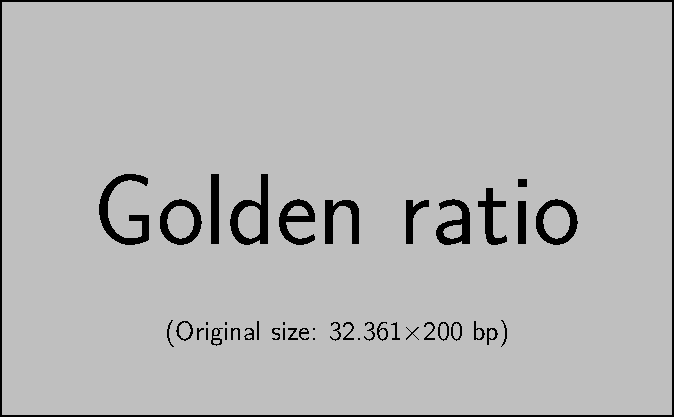
\includegraphics{placeholder_images/example-image-golden.pdf}
    \caption[Desirability index of various \glsfmtshort{rom}s]{A radar chart
        showing various the performance of various models compared against a
    desirability index (scale) sought after in all \glsfmtlong{rom}s}
    \label{fig:spiderdiagram}
\end{figure}


From~\cref{fig:spiderdiagram}, it is evident  that all physics-based \glspl{rom}
presented thus far entail extensive  parametrisation efforts \fxnote{at the end,
count  and  substitute  the  canonical  number of  parameters  here}  to  render
them  suitable for  a practical  application. The  difficulties associated  with
such  parametrisation,  coupled  with  inherent uncertainties  in  the  obtained
parameter values act  as a strong deterrent to stakeholders  outside academia to
adopt  physics-based  models for  online  implementation  in a  \gls{bms}.  This
motivates the  need for even  further simplified physics-based models.  One such
modelling  candidate  is briefly  introduced  next  and  is analysed  in  detail
in~\cref{ch:spmanalysis}.


Haran~\etal{}~\cite{Haran1998}  proposed a  highly simplified  representation of
porous  electrodes for  the metal  hydride cell  chemistry. In  this work,  each
porous electrode  was represented as  a single spherical particle.  This concept
was adopted for lithium ion batteries  by Ning and Popov~\cite{Ning2004} and has
since  become quite  popular.  Models employing  this  lumped representation  of
electrodes are referred to as  \glsfmtlong{spm}s (\gls{spm}s). These models have
three advantages. Since they involve only a subset of parameters of the original
\gls{dfn} model,  most of them being  geometric quantities that can  be directly
measured  without  extensive chemical  or  electrical  testing, \glspl{spm}  are
easier to parametrise than other physics-based reduced order model. Furthermore,
they  are computationally  cheap, especially  when coupled  with the  polynomial
approximation  for solving  the  solid diffusion  equation  for each  electrode.
Finally, all model parameters in  the \gls{spm} retain their physical character,
aiding in  a direct and  intuitive understanding  of physical parameters  on the
cell's operation.

This concludes  the author's review of  literature of the various  reduced order
modelling  strategies. Based  on the  wealth  of information  gleaned from  this
study,  it was  possible to  make  an informed  choice to  pursue the  \gls{spm}
approach  for further  research.  In particular,  it came  to  light that  there
has  been  no systematic  analysis  of  the  state  of the  art  \gls{spm}-based
approach with  a view  to quantify their  performance boundaries.  This author's
contributions to  the time-domain  implementation-focus reduced  order modelling
field include
\begin{itemize}[noitemsep,topsep=0pt, before={\vspace*{-0.25\baselineskip}}]
    \item a thorough analysis of the existing \gls{spm} variants ranging from the rudimentary to the sophisticated
    \item enumeration of issues plaguing each \gls{spm} variant, including current state of the art
    \item study of further literature on the current tactics to overcome the current challenges along with their associated drawbacks
    \item conducting a  wide range of hypotheses-driven trials in an attempt to enhance  the basic \gls{spm} (some of which did not yield the desired
        improvements), and
    \item arriving at  a  feasible  approach  capable  of  moulding  the
        \gls{spm}  framework into  a  readily implementable  solution in
        electric vehicle applications
\end{itemize}
This research was  performed through an iterative cycle of  analysis, design and
simulation-based verification  and shall be  elucidated in a  discourse spanning
two chapters \viz{} \cref{ch:spmanalysis} and~\cref{ch:newelectrolytemodel}.


